% !TeX root = ../main.tex

\newlecture[The Capital Asset Pricing Model (CAPM)][Nov 19, 2026]

\header{Market Equilibrium}
Under the one-fund theorem, everyone buys the \dbb{same single fund} of risky assets. What is that fund?
\keypoint{Answer: \rb{the market portfolio}!}
\begin{definition}[\rb{Market Portfolio}]
    A portfolio of every stock in the market, held in proportion to that stock's representation in the entire market.
\end{definition}
Why: if everyone holds the same fund $F$, then adding up all investors' holdings, the total demand for each stock is in the proportions of $F$. In equilibrium, demand equals what exists in the market, so $F$ must be the market.

\heading{Computation of the Market Portfolio}
Each asset's weight in the market portfolio is its share of the market's total value:
\[\boxed{w_i = \frac{\$\text{ value of asset } i}{\$\text{ value of market}}}\]
These weights are called \rb{capitalization weights}, where capitalization $=$ shares outstanding $\times$ price.

\begin{example}
    \b{Given}: three securities.
    \begin{center}
    \begin{tabular}{lcc}
        \toprule
        Security & Shares outstanding & Price (\$)\\
        \midrule
        Jazz & 10,000 & 6\\
        Classical & 30,000 & 4\\
        Rock & 40,000 & 5.5\\
        \bottomrule
    \end{tabular}
    \end{center}
    \b{Find}: the market portfolio weights.

    \b{Solution}: capitalization $=$ shares $\times$ price, then divide by the total.
    \begin{center}
    \begin{tabular}{lcc}
        \toprule
        Security & Capitalization & Weight\\
        \midrule
        Jazz & $10{,}000 \times 6 = 60{,}000$ & $60/400 = 3/20$\\
        Classical & $30{,}000 \times 4 = 120{,}000$ & $120/400 = 3/10$\\
        Rock & $40{,}000 \times 5.5 = 220{,}000$ & $220/400 = 11/20$\\
        \midrule
        Total & 400,000 & 1\\
        \bottomrule
    \end{tabular}
    \end{center}
    \begin{center}
    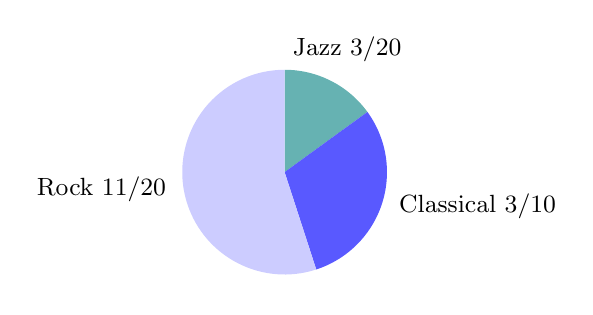
\begin{tikzpicture}
        \fill[teal!60] (0,0) -- (90:1.3) arc (90:36:1.3) -- cycle;
        \fill[blue!65] (0,0) -- (36:1.3) arc (36:-72:1.3) -- cycle;
        \fill[blue!20] (0,0) -- (-72:1.3) arc (-72:-270:1.3) -- cycle;
        \node at (63:1.75) {\small Jazz 3/20};
        \node[right] at (-18:1.4) {\small Classical 3/10};
        \node[left] at (-171:1.4) {\small Rock 11/20};
    \end{tikzpicture}
    \end{center}
\end{example}

\heading{The Capital Market Line}
With the market portfolio $M$ as the one fund, the efficient frontier is the line from $r_f$ through $M$:
\[\boxed{\overline{r} = r_f + \left(\frac{\overline{r}_M - r_f}{\sigma_M}\right)\sigma}\]
This is the \rb{capital market line} (CML). Its slope $\dfrac{\overline{r}_M - r_f}{\sigma_M}$ is often called the \rb{price of risk}: the extra mean return you get per unit of standard deviation.
\begin{center}
\begin{tikzpicture}[x=1.5cm, y=1.15cm]
    \pgfmathsetmacro{\m}{sqrt(0.49 + 0.4)}
    \pgfmathsetmacro{\rM}{1.9 + 1/(2.5*0.7)}
    \pgfmathsetmacro{\sM}{sqrt(1 + 2.5*(\rM-1.9)^2)}
    \draw[->] (0,0) -- (4.4,0) node[right] {$\sigma$};
    \draw[->] (0,0) -- (0,4.2) node[above] {$\overline{r}$};
    \draw[thick, domain=0.25:3.8, samples=60, smooth, variable=\r] plot ({sqrt(1 + 2.5*(\r-1.9)^2)}, {\r});
    \draw[very thick, ->] (0,1.2) -- (3.0,{1.2 + 3.0*\m}) node[above left] {CML};
    \draw (0.08,1.2) -- (-0.08,1.2) node[left] {$r_f$};
    \draw[dotted] (0,\rM) node[left] {$\overline{r}_M$} -- (\sM,\rM) -- (\sM,0) node[below] {$\sigma_M$};
    \fill[red!70!black] (\sM,\rM) circle (2.2pt) node[below right] {$M$};
\end{tikzpicture}
\end{center}

\begin{example}
    \b{Given}: $r_f = 0.05$, $\overline{r}_M = 0.12$, $\sigma_M = 0.15$.

    \b{Find}: you would like to earn 20\% on average. What will be the standard deviation of your portfolio?

    \b{Solution}: you want your portfolio to lie on the CML (the least risk for that mean), so
    \[0.20 = 0.05 + \frac{0.12 - 0.05}{0.15}\,\sigma \quad \Rightarrow \quad \boxed{\sigma = 0.3214}\]
    Since $\sigma > \sigma_M$, this point is beyond $M$ on the CML. Its standard deviation is $(1-\alpha)\sigma_M$, so $1 - \alpha = 0.3214/0.15 = 2.14$: invest 214\% of your money in the market by \dbb{borrowing} 114\% at $r_f$.
\end{example}

\header{The Capital Asset Pricing Model}
\b{Assumptions}:
\begin{enumerate}[label=(\arabic*)]
    \item All investors are Markowitz mean-variance investors.
    \item Short selling is allowed.
    \item There exists a risk-free asset.
    \item Investors share the same predictions of means, variances and covariances.
\end{enumerate}
\begin{framed}
    \textbf{Theorem} (\rb{Capital Asset Pricing Model}). If the market portfolio $M$ is efficient, the expected return $\overline{r}_i$ of any asset $i$ satisfies
    \[\boxed{\overline{r}_i - r_f = \beta_i(\overline{r}_M - r_f), \qquad \text{where } \beta_i = \frac{\sigma_{iM}}{\sigma_M^2}}\]
\end{framed}
Here $\overline{r}_i - r_f$ is the asset's \dbb{excess return} and $\overline{r}_M - r_f$ is the market's excess return (the \dbb{market risk premium}).

\heading{Proof of CAPM}
Consider a portfolio with weight $\alpha$ in asset $i$ and $1-\alpha$ in the market portfolio. As $\alpha$ varies, it traces the dotted curve through $i$ and $M$:
\begin{center}
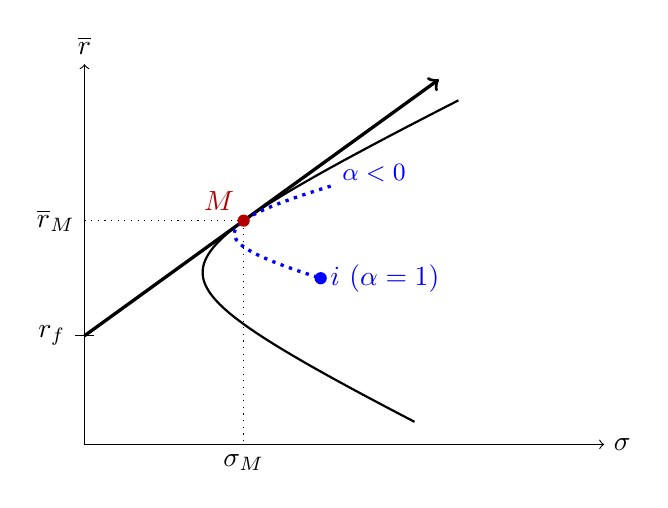
\begin{tikzpicture}[x=1.5cm, y=1.15cm]
    \pgfmathsetmacro{\m}{sqrt(0.49 + 0.4)}
    \pgfmathsetmacro{\rM}{1.9 + 1/(2.5*0.7)}
    \pgfmathsetmacro{\sM}{sqrt(1 + 2.5*(\rM-1.9)^2)}
    \pgfmathsetmacro{\ri}{1.2 + 0.5*(\rM - 1.2)}
    \pgfmathsetmacro{\siM}{0.5*\sM*\sM}
    \draw[->] (0,0) -- (4.4,0) node[right] {$\sigma$};
    \draw[->] (0,0) -- (0,4.2) node[above] {$\overline{r}$};
    \draw[thick, domain=0.25:3.8, samples=60, smooth, variable=\r] plot ({sqrt(1 + 2.5*(\r-1.9)^2)}, {\r});
    \draw[very thick, ->] (0,1.2) -- (3.0,{1.2 + 3.0*\m});
    \draw (0.08,1.2) -- (-0.08,1.2) node[left] {$r_f$};
    \draw[very thick, dotted, blue, domain=-0.6:1, samples=60, smooth, variable=\a]
        plot ({sqrt(\a*\a*4 + 2*\a*(1-\a)*\siM + (1-\a)*(1-\a)*\sM*\sM)}, {\a*\ri + (1-\a)*\rM});
    \draw[dotted] (0,\rM) node[left] {$\overline{r}_M$} -- (\sM,\rM) -- (\sM,0) node[below] {$\sigma_M$};
    \fill[red!70!black] (\sM,\rM) circle (2.2pt) node[above left] {$M$};
    \fill[blue] (2,\ri) circle (2.2pt) node[right] {$i$ ($\alpha = 1$)};
    \node[blue, right] at (2.1,3.0) {\small $\alpha < 0$};
\end{tikzpicture}
\end{center}
Using the variance trick:
\[\overline{r}_\alpha = \alpha\overline{r}_i + (1-\alpha)\overline{r}_M, \qquad \sigma_\alpha = \sqrt{\alpha^2\sigma_i^2 + 2\alpha(1-\alpha)\sigma_{iM} + (1-\alpha)^2\sigma_M^2}\]
\b{Key idea}: at $\alpha = 0$ the portfolio \ul{is} $M$. The curve can't cross the CML (nothing feasible lies above the efficient frontier), so at $\alpha = 0$ the curve and the CML are \rb{tangent}: they have the same slope.

\b{Slope of the CML}: $\dfrac{\overline{r}_M - r_f}{\sigma_M}$.

\b{Slope of the curve at $\alpha = 0$} (chain rule):
\[\left.\frac{d\overline{r}_\alpha}{d\sigma_\alpha}\right|_{\alpha=0} = \left.\left(\frac{d\overline{r}_\alpha}{d\alpha}\right)\left(\frac{d\alpha}{d\sigma_\alpha}\right)\right|_{\alpha=0} = \left.\left(\frac{d\overline{r}_\alpha}{d\alpha}\right)\left(\frac{d\sigma_\alpha}{d\alpha}\right)^{-1}\right|_{\alpha=0}\]
\begin{itemize}
    \item $\left.\dfrac{d\overline{r}_\alpha}{d\alpha}\right|_{\alpha=0} = \overline{r}_i - \overline{r}_M$
    \item $\left.\dfrac{d\sigma_\alpha}{d\alpha}\right|_{\alpha=0} = \left.\dfrac{\alpha\sigma_i^2 + (1-2\alpha)\sigma_{iM} + (\alpha-1)\sigma_M^2}{\sigma_\alpha}\right|_{\alpha=0} = \dfrac{\sigma_{iM} - \sigma_M^2}{\sigma_M}$ \quad (since $\sigma_{\alpha=0} = \sigma_M$)
\end{itemize}
So
\[\left.\frac{d\overline{r}_\alpha}{d\sigma_\alpha}\right|_{\alpha=0} = \frac{(\overline{r}_i - \overline{r}_M)\sigma_M}{\sigma_{iM} - \sigma_M^2}\]
\b{Set the slopes equal}:
\[\frac{(\overline{r}_i - \overline{r}_M)\sigma_M}{\sigma_{iM} - \sigma_M^2} = \frac{\overline{r}_M - r_f}{\sigma_M} \quad \Rightarrow \quad \overline{r}_i - \overline{r}_M = \frac{(\overline{r}_M - r_f)(\sigma_{iM} - \sigma_M^2)}{\sigma_M^2} = (\overline{r}_M - r_f)\left(\frac{\sigma_{iM}}{\sigma_M^2} - 1\right)\]
Add $\overline{r}_M - r_f$ to both sides:
\[\overline{r}_i - r_f = \frac{\sigma_{iM}}{\sigma_M^2}(\overline{r}_M - r_f) \quad \Rightarrow \quad \overline{r}_i = r_f + \beta_i(\overline{r}_M - r_f), \quad \beta_i = \frac{\sigma_{iM}}{\sigma_M^2} \qquad \blacksquare\]

\begin{example}
    \b{Given}: $r_f = 8\%$, $(\overline{r}_M, \sigma_M) = (12\%, 15\%)$, and an asset whose covariance with the market is $\sigma_{iM} = 0.045$.

    \b{Find}: the expected return on the asset.

    \b{Solution}: use CAPM. First compute beta:
    \[\beta_i = \frac{\sigma_{iM}}{\sigma_M^2} = \frac{0.045}{(0.15)^2} = 2.0\]
    \[\overline{r}_i = r_f + \beta_i(\overline{r}_M - r_f) = 0.08 + 2(0.12 - 0.08) = \boxed{0.16}\]
\end{example}

\header{Consequences of CAPM}
\heading{The Security Market Line}
Plotting CAPM as expected return against $\beta$ gives a straight line, the \rb{security market line} (SML):
\begin{center}
\begin{tikzpicture}
    \draw[->] (0,0) -- (5.6,0) node[right] {$\beta$};
    \draw[->] (0,0) -- (0,3.4) node[above] {$\overline{r}$};
    \draw[very thick, dashed, blue] (0,0.8) -- (5.2,3.2);
    \draw (0.08,0.8) -- (-0.08,0.8) node[left] {$r_f$};
    \draw[dotted] (0,{0.8+2.4*2.5/5.2}) node[left] {$\overline{r}_M$} -- (2.5,{0.8+2.4*2.5/5.2}) -- (2.5,0) node[below] {$\beta = 1$};
    \fill[red!70!black] (2.5,{0.8+2.4*2.5/5.2}) circle (2pt) node[above left] {$M$};
    \node[blue, below right] at (3.6,2.3) {\small security market line};
\end{tikzpicture}
\end{center}
\keypoint{\rb{All securities lie along this line}: $\overline{r}_i = r_f + \beta_i(\overline{r}_M - r_f)$.}
Compare with the CML: the CML plots against $\sigma$ and only \ul{efficient} portfolios lie on it. The SML plots against $\beta$ and \ul{every} asset or portfolio lies on it.

\b{Correlation with the market ($\beta$) determines your expected return}:
\begin{center}
\begin{tabular}{lll}
    $\beta_i = 0$ & $\Rightarrow \overline{r}_i = r_f + 0(\overline{r}_M - r_f) = r_f$ & risk-free rate\\
    $\beta_i = 1$ & $\Rightarrow \overline{r}_i = r_f + 1(\overline{r}_M - r_f) = \overline{r}_M$ & market return!\\
    $\beta_i = 2$ & $\Rightarrow \overline{r}_i = r_f + 2(\overline{r}_M - r_f) = 2\overline{r}_M - r_f$ & etc.
\end{tabular}
\end{center}

\b{$\beta$ also determines expected movement with the market}: $\overline{r}_i - r_f = \beta_i(\overline{r}_M - r_f)$. E.g.\ with $\beta_i = 2$, $\overline{r}_i - r_f = 2(\overline{r}_M - r_f)$: if the market is up, you expect to be up \dbb{twice as much}; if the market is down, you expect to be down twice as much.

Real examples (2000--2005): Microsoft (MSFT) had $\beta = 1.26$, moving with the Nasdaq more than one-for-one. ACM Income Fund (ACG) had $\beta = -0.04$, essentially unrelated to (even slightly against) the S\&P 500.

\heading{Risk and CAPM}
CAPM gives the expected return $\overline{r}_i = r_f + \beta_i(\overline{r}_M - r_f)$, so the actual (random) return can be written
\[r_i = r_f + \beta_i(r_M - r_f) + \varepsilon_i, \qquad E(\varepsilon_i) = 0\]
\b{Claim}: $\varepsilon_i$ is uncorrelated with the market. Take covariance with $r_M$, using the trick (constants like $r_f$ drop out):
\begin{align*}
    \operatorname{cov}(r_i, r_M) &= \operatorname{cov}\left(r_f + \beta_i(r_M - r_f) + \varepsilon_i,\ r_M\right)\\
    &= \underbrace{\operatorname{cov}(r_f, r_M)}_{0} + \beta_i\operatorname{cov}(r_M, r_M) - \underbrace{\beta_i\operatorname{cov}(r_f, r_M)}_{0} + \operatorname{cov}(\varepsilon_i, r_M)\\
    &= \beta_i\sigma_M^2 + \operatorname{cov}(\varepsilon_i, r_M)
\end{align*}
But $\beta_i\sigma_M^2 = \frac{\sigma_{iM}}{\sigma_M^2}\sigma_M^2 = \sigma_{iM} = \operatorname{cov}(r_i, r_M)$. So $\operatorname{cov}(r_i, r_M) = \operatorname{cov}(r_i, r_M) + \operatorname{cov}(\varepsilon_i, r_M)$, which gives
\keypoint{$\operatorname{cov}(\varepsilon_i, r_M) = 0$: \rb{$\varepsilon_i$ is uncorrelated with the market!}}

\heading{The Variance of an Asset}
\begin{align*}
    \sigma_i^2 = \operatorname{cov}(r_i, r_i) &= \operatorname{cov}\left(r_f + \beta_i(r_M - r_f) + \varepsilon_i,\ r_f + \beta_i(r_M - r_f) + \varepsilon_i\right)\\
    &= \beta_i^2\operatorname{var}(r_M) + 2\beta_i\underbrace{\operatorname{cov}(r_M, \varepsilon_i)}_{0} + \operatorname{var}(\varepsilon_i) = \boxed{\beta_i^2\sigma_M^2 + \operatorname{var}(\varepsilon_i)}
\end{align*}
The risk in $r_i$ is the sum of two parts:
\begin{enumerate}[label=(\arabic*)]
    \item $\beta_i^2\sigma_M^2$: \rb{systematic risk}, associated with the market as a whole.
    \item $\operatorname{var}(\varepsilon_i)$: \rb{nonsystematic} (idiosyncratic, specific) risk. It is uncorrelated with the market and \dbb{can be reduced by diversification}.
\end{enumerate}

\heading{Summary of CAPM Equations}
\keypoint{\begin{tabular}{rl}
    Returns: & $r_i = r_f + \beta_i(r_M - r_f) + \varepsilon_i$\\
    & where $E(\varepsilon_i) = 0$, $\operatorname{cov}(r_M, \varepsilon_i) = 0$\\[4pt]
    Mean returns (reward): & $\overline{r}_i = r_f + \beta_i(\overline{r}_M - r_f)$\\[4pt]
    Variances (risk): & $\sigma_i^2 = \beta_i^2\sigma_M^2 + \operatorname{var}(\varepsilon_i)$
\end{tabular}}
Expected return is determined \ul{not by the variance} of an asset or portfolio, but \ul{only by its beta}, which measures the amount of risk coming from the market portfolio. These equations govern the risk/reward relationship.

\begin{center}
\begin{tikzpicture}[x=1.5cm, y=1.15cm]
    \pgfmathsetmacro{\m}{sqrt(0.49 + 0.4)}
    \pgfmathsetmacro{\rM}{1.9 + 1/(2.5*0.7)}
    \pgfmathsetmacro{\sM}{sqrt(1 + 2.5*(\rM-1.9)^2)}
    \draw[->] (0,0) -- (4.4,0) node[right] {$\sigma$};
    \draw[->] (0,0) -- (0,4.2) node[above] {$\overline{r}$};
    \draw[thick, domain=0.25:3.8, samples=60, smooth, variable=\r] plot ({sqrt(1 + 2.5*(\r-1.9)^2)}, {\r});
    \draw[very thick, ->] (0,1.2) -- (3.0,{1.2 + 3.0*\m});
    \draw (0.08,1.2) -- (-0.08,1.2) node[left] {$r_f$};
    \fill[red!70!black] (\sM,\rM) circle (2.2pt) node[above left] {$M$};
    \fill[blue] (2.4,1.9) circle (2.2pt) node[right] {$i$};
    \draw[->, dashed, green!50!black, thick] (-0.9,0.6) -- (-0.9,3.6) node[above, align=center] {\small reward:\\[-2pt]\small $\beta_i$};
    \draw[->, dashed, red!70!black, thick] (1.0,-0.7) -- (3.8,-0.7) node[right, align=left] {\small risk: $\beta_i^2\sigma_M^2$\\[-2pt]\small $+ \operatorname{var}(\varepsilon_i)$};
\end{tikzpicture}
\end{center}
Asset $i$ sits to the right of the CML because of its nonsystematic risk $\operatorname{var}(\varepsilon_i)$. That extra risk adds to $\sigma_i$ but earns no extra mean return.

\heading{Implications of CAPM}
\begin{itemize}
    \item[$\rightarrow$] According to the theory, the only portfolio of risky assets you should hold is \rb{the market}.
    \item[$\rightarrow$] Hence, you are only rewarded (with expected return) for risk \ul{related to the market}.
    \item[$\rightarrow$] That risk is measured by \rb{$\beta$}, not by the variance of your asset.
    \item[$\rightarrow$] The return on an asset is determined by \dbb{how it fits into the market portfolio}, not by its characteristics alone.
\end{itemize}

\heading{Portfolio and Security Risk}
\begin{itemize}
    \item We started at the \b{portfolio level}: Markowitz theory minimized risk (variance) in optimal portfolios, and risk was measured by portfolio variance.
    \item We arrived at the \b{security level}: CAPM says risk is given by beta. In fact, CAPM says beta is the appropriate measure at \ul{any} level, security or portfolio.
\end{itemize}

\heading{The Big Picture of CAPM}
We were looking for a theory relating risk and return for assets, something like ``\dbb{expected return is determined solely by risk}''. But what do we mean by risk?
\begin{center}
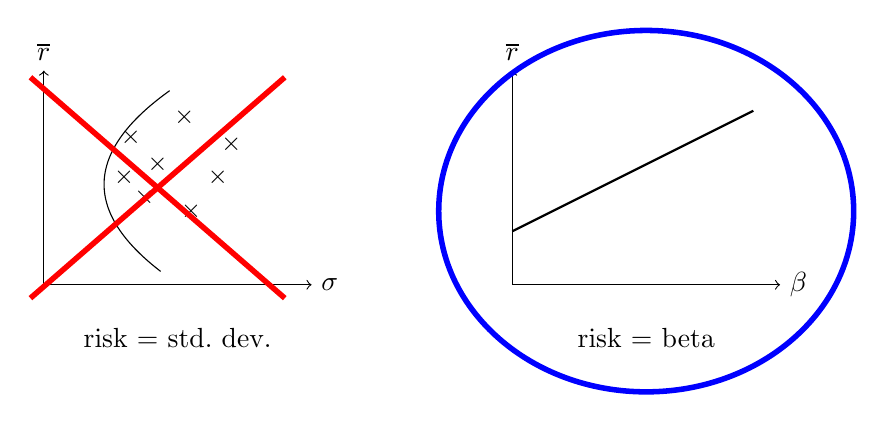
\begin{tikzpicture}[scale=0.85]
    % left: risk = std dev (crossed out)
    \draw[->] (0,0) -- (4,0) node[right] {$\sigma$};
    \draw[->] (0,0) -- (0,3.2) node[above] {$\overline{r}$};
    \draw[domain=0.2:2.9, samples=40, smooth, variable=\r] plot ({0.9 + 0.5*(\r-1.5)^2}, {\r});
    \foreach \x/\y in {1.3/2.2, 2.1/2.5, 1.7/1.8, 2.6/1.6, 1.5/1.3, 2.2/1.1, 2.8/2.1, 1.2/1.6} { \node at (\x,\y) {\small $\times$}; }
    \draw[red, line width=2pt] (-0.2,-0.2) -- (3.6,3.1);
    \draw[red, line width=2pt] (-0.2,3.1) -- (3.6,-0.2);
    \node at (2,-0.8) {risk $=$ std.\ dev.};
    % right: risk = beta (circled)
    \begin{scope}[xshift=7cm]
        \draw[->] (0,0) -- (4,0) node[right] {$\beta$};
        \draw[->] (0,0) -- (0,3.2) node[above] {$\overline{r}$};
        \draw[thick] (0,0.8) -- (3.6,2.6);
        \node at (2,-0.8) {risk $=$ beta};
        \draw[blue, line width=2pt] (2.0,1.1) ellipse (3.1 and 2.7);
    \end{scope}
\end{tikzpicture}
\end{center}
Against standard deviation, assets are scattered with no single relationship. Against beta, they all lie on one line (the SML).

\heading{Beta of a Portfolio}
Given a portfolio $r_p = w_1r_1 + \cdots + w_nr_n$, what is $\beta_p$? Covariance is linear in each argument:
\begin{align*}
    \beta_p = \frac{\operatorname{cov}(r_p, r_M)}{\operatorname{var}(r_M)} &= \frac{\operatorname{cov}(w_1r_1 + \cdots + w_nr_n,\ r_M)}{\operatorname{var}(r_M)}\\
    &= \frac{w_1\operatorname{cov}(r_1, r_M) + \cdots + w_n\operatorname{cov}(r_n, r_M)}{\operatorname{var}(r_M)} = \boxed{w_1\beta_1 + \cdots + w_n\beta_n}
\end{align*}
\keypoint{The beta of a portfolio is the \rb{weighted average of the betas} (just like portfolio mean return).}
